% ============================================================
% CHAPTER 6: BACKEND SYSTEM ARCHITECTURE AND IMPLEMENTATION
% AgriVerify --- AI-Powered Seed Quality Assessment and Farmer Feedback System
% ============================================================
Our backend application coordinates request routing, database state, and downstream machine learning inference. We built the service using ASP.NET Core on .NET 8, organizing the code around Clean Architecture principles. This separation ensures that core business logic remains independent of external databases and third-party APIs.

Isolating the database configuration and external API adapters from the domain entities allowed us to develop the system incrementally. For example, during testing, we could swap out the cloud-based SQL Server configuration for an in-memory database instance without altering the service logic that runs the seed verification rules.

% ============================================================
\section{Architectural Design}
\label{sec:backend-architecture}
% ============================================================

The backend uses four distinct projects corresponding to the layers in Figure~\ref{fig:backend-clean-architecture}. Dependencies flow inward, meaning inner projects cannot reference outer ones. This compile-time constraint prevents database or presentation concerns from leaking into the core logic.

\begin{figure}[H]
\centering
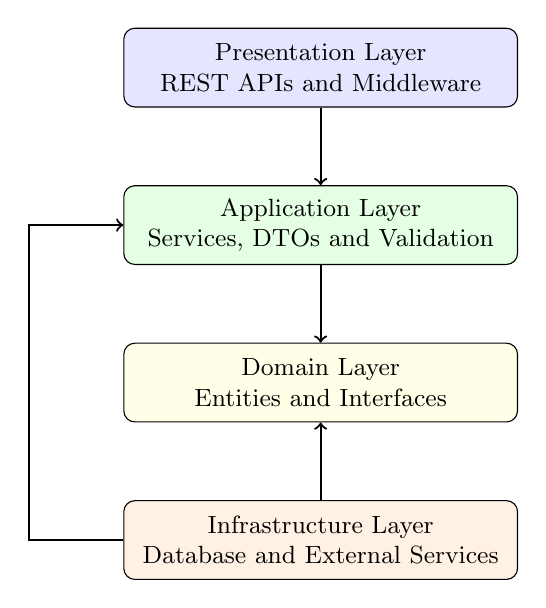
\begin{tikzpicture}[
node distance=2cm,
every node/.style={
draw,
rounded corners,
minimum width=5cm,
minimum height=1cm,
align=center,
font=\small
}
]
\node[fill=blue!10] (api) {Presentation Layer\\REST APIs and Middleware};
\node[fill=green!10, below of=api] (application) {Application Layer\\Services, DTOs and Validation};
\node[fill=yellow!10, below of=application] (domain) {Domain Layer\\Entities and Interfaces};
\node[fill=orange!10, below of=domain] (infra) {Infrastructure Layer\\Database and External Services};
\draw[->, thick] (api) -- (application);
\draw[->, thick] (application) -- (domain);
\draw[->, thick] (infra) -- (domain);
\draw[->, thick] (infra.west) -- ++(-1.2cm,0) |- (application.west);

\end{tikzpicture}
\caption{Backend Clean Architecture Layers}
\label{fig:backend-clean-architecture}
\end{figure}

This physical separation simplifies testing. When writing unit tests for our verification logic, we mocked the repository interfaces and simulated image analysis runs offline without needing active connections to Azure or SQL Server. It also helps with deployment; we can scale the API presentation layer on serverless containers during peak harvesting seasons while leaving the underlying database server on a fixed tier to control costs.

% ============================================================
\section{Technology Stack}
\label{sec:backend-tech-stack}
% ============================================================

The backend uses specific libraries and frameworks to support request handling, user session management, and external service client interfaces. The core components of this technology stack are outlined in Table~\ref{tab:backend-tech-stack}.

\begin{table}[htbp]
\centering
\caption{Backend Technology Stack}
\label{tab:backend-tech-stack}
\small
\renewcommand{\arraystretch}{1.1}

\begin{tabularx}{\textwidth}{|p{5.2cm}|X|}
\hline
\textbf{Technology} & \textbf{Purpose} \\
\hline
ASP.NET Core Web API & Backend API framework \\
\hline
C\char35{} and .NET 8 & Backend programming environment \\
\hline
Entity Framework Core & Database ORM and migrations \\
\hline
SQL Server & Relational database management \\
\hline
JWT Authentication & Secure user authentication \\
\hline
ASP.NET Core Identity & User and role management \\
\hline
Azure OCR & Text extraction from seed packets \\
\hline
Azure OpenAI & AI-generated explanations \\
\hline
Azure Blob Storage & Cloud image storage \\
\hline
FluentValidation & Input validation \\
\hline
AutoMapper & DTO mapping \\
\hline
Swagger & API documentation \\
\hline
Serilog & Request logging and monitoring \\
\hline
\end{tabularx}
\end{table}

Choosing ASP.NET Core was driven by its Kestrel web server performance and built-in asynchronous pipeline. Handling multi-part form data uploads for 300KB images requires non-blocking I/O thread management, otherwise, simultaneous uploads from multiple farmers would exhaust the server's thread pool. For data persistence, Entity Framework Core serves as our database adapter. Using code-first migrations automated schema updates as we added fields for DUS morphological properties, avoiding the need to run manual SQL alter scripts across development and production environments.

% ============================================================
\section{Project Structure}
\label{sec:backend-project-structure}
% ============================================================

We organized the backend source code into distinct physical folders to maintain responsibility boundaries across the architecture, as detailed in Table~\ref{tab:backend-project-structure}.

\begin{table}[htbp]
\centering
\caption{Backend Project Structure}
\label{tab:backend-project-structure}
\small
\renewcommand{\arraystretch}{1.1}

\begin{tabularx}{\textwidth}{|p{5.2cm}|X|}
\hline
\textbf{Folder / Layer} & \textbf{Purpose} \\
\hline
Domain & Business entities and interfaces \\
\hline
Application & Services, DTOs and validation \\
\hline
Infrastructure & Database and cloud integrations \\
\hline
Presentation & API controllers and middleware \\
\hline
Persistence & Repositories and migrations \\
\hline
Services & AI and Azure integrations \\
\hline
Configurations & Application configuration files \\
\hline
Middleware & Authentication and exception handling \\
\hline
\end{tabularx}
\end{table}

By structuring the solution into separate projects, the .NET compiler enforces our architectural boundaries. The Domain project compile target has zero dependencies. The Application project, containing the business interface definitions, references only Domain. Concrete implementations—like EF Core context classes, Azure SDK integrations, and controller routes—reside in the Infrastructure and Presentation projects respectively, preventing presentation details from dictating business structures.

% ============================================================
\section{Domain Layer}
\label{sec:domain-layer}
% ============================================================

The Domain Layer contains the application's core data models and interface contracts. This project has zero dependencies on external storage libraries, web frameworks, or ORM tools, ensuring that our agricultural verification rules remain isolated from infrastructure changes.

\subsection{Core Entities}
Our domain models map the physical elements of the seed verification workflow to structured data definitions. The \texttt{User} base class integrates with ASP.NET Core Identity to handle authentication, but we extended it with a one-to-one relationship to a \texttt{Profile} entity storing regional details (like District and Phone) to support geographic query filtering by agricultural officers. The physical components are modeled through \texttt{Seed} (defining reference cultivars) and \texttt{SeedBatch} (representing physical seed batches distributed by manufacturers). 

When a verification scan is processed, the system creates a \texttt{DetectionResult} containing model labels, confidence levels, and physical parameters. If a farmer reports an issue with a seed batch, a \texttt{Complaint} entity is generated to track the investigation details. Lastly, we log system actions through the \texttt{AuditLog} entity to maintain a clear record of administrative and verification changes.

\subsection{Interfaces}
Rather than allowing the business logic to directly call SQL Server or Azure services, we defined interfaces within the Domain layer. These include repository abstractions like \texttt{IRepository<T>} and functional service interfaces like \texttt{IVerificationService} and \texttt{IComplaintService}. During unit testing, this allowed us to substitute the live cloud integrations with mock classes, meaning we could test the verification routing and database mappings locally without paying for Azure consumption or relying on active internet access.

% ============================================================
\section{Application Layer}
\label{sec:application-layer}
% ============================================================

The Application Layer coordinates the business workflows and transaction boundaries of the platform.

\subsection{Application Services}
The Application layer houses the coordinate logic for the system's workflows. The \texttt{VerificationService} handles the steps of the analysis pipeline: validating file parameters, calling the FastAPI model service, uploading the raw image to blob storage, and invoking Azure OpenAI to parse the combined metrics. By placing this coordination in a dedicated service, we kept the API controllers small. Other services include \texttt{ComplaintService}, which validates farmer complaints and routes them to regional officer queues based on district IDs, and \texttt{AuthenticationService}, which handles BCrypt password validation and issues JWT tokens.

\subsection{DTOs}
Passing raw Entity Framework models directly to the client creates two issues: it exposes our internal database schema, and it causes serialization cycles due to navigation properties (for instance, a User referencing a Complaint that references a User). To prevent this, we mapped database entities to Data Transfer Objects (DTOs) using AutoMapper. For example, \texttt{VerificationResponse} only returns the visual classification label, confidence score, and extracted DUS metrics, stripping out internal SQL primary keys and auditing properties. Using DTOs also reduced JSON payload sizes, which is important for mobile users operating on high-latency rural connections. The primary DTOs utilized in the system and their respective purposes are listed in Table~\ref{tab:important-dtos}.

\begin{table}[htbp]
\centering
\caption{Important DTOs}
\label{tab:important-dtos}
\small
\renewcommand{\arraystretch}{1.1}

\begin{tabularx}{\textwidth}{|p{5.2cm}|X|}
\hline
\textbf{DTO} & \textbf{Purpose} \\
\hline
VerificationRequest & Seed verification request \\
\hline
VerificationResponse & AI verification result \\
\hline
LoginRequest & User login request \\
\hline
AuthResponse & JWT authentication response \\
\hline
CreateComplaintRequest & Complaint submission \\
\hline
OfficerDto & Officer information \\
\hline
AdminDashboardResponse & Dashboard statistics \\
\hline
\end{tabularx}
\end{table}

\subsection{Validation}
To prevent malformed data from hitting the deep learning container or database, we write validation logic using FluentValidation. We intercept incoming requests before they reach the main service logic. The validator checks that uploaded files have a valid MIME type (restricting uploads to JPEG or PNG), verifies that the payload does not exceed the 10MB server limit (though client-side compression usually keeps it under 300KB), and enforces password and email syntax constraints. This preemptive validation prevents downstream errors in the PyTorch model service and saves database connections.

% ============================================================
\section{Infrastructure Layer}
\label{sec:infrastructure-layer}
% ============================================================

The Infrastructure Layer implements the interfaces defined in our Domain layer, handling direct database connections and network communication with external APIs.

\subsection{Database Management and Repositories}
Database communication is configured using EF Core. While ORMs simplify basic database updates, they can introduce performance bottlenecks if queries are not carefully constructed. For example, to avoid the N+1 query problem—where the application executes a separate SQL query to load the user profile for every verification record displayed on the officer dashboard—we wrote optimized LINQ queries using \texttt{.Include()} statements. This forces EF Core to generate single SQL JOIN queries, returning all required data in one database trip. We also implemented the repository pattern to encapsulate these data access details behind the domain interfaces, keeping database-specific LINQ logic out of the application services. We use EF code-first migrations to apply schema updates incrementally, keeping development and production databases synchronized.

\subsection{AI and Cloud Integrations}
Our infrastructure implementations handle connection lifecycles for external cloud APIs. The external service integrations are detailed in Table~\ref{tab:external-services}.

\begin{table}[htbp]
\centering
\caption{External Service Integrations}
\label{tab:external-services}
\small
\renewcommand{\arraystretch}{1.1}

\begin{tabularx}{\textwidth}{|p{5.2cm}|X|}
\hline
\textbf{Service} & \textbf{Purpose} \\
\hline
Azure OCR & Text extraction from seed packets \\
\hline
Azure OpenAI & AI-generated recommendations \\
\hline
Azure Blob Storage & Cloud image storage \\
\hline
ResNet Model & Paddy seed Quality Determination\\
\hline
\end{tabularx}
\end{table}

When the verification service receives a compressed image, the storage adapter uploads it to Azure Blob Storage and generates a read-only URL. This URL is dispatched to the Azure AI Vision OCR service to extract text from the packaging label, such as batch numbers and expiry dates. At the same time, the image is sent to our FastAPI service hosting the ResNet50 model. The results are aggregated, and the backend sends the combined data to the Azure OpenAI service, instructing the model to synthesize the raw statistics and OCR text into a plain-language summary for Meitei farmers.

% ============================================================
\section{Database Schema}
\label{sec:database-schema}
% ============================================================

The backend database maintains relationships between users, verification results, complaints, and audit records. The database schema and its corresponding primary/foreign key mappings are represented in the Entity-Relationship Diagram in Figure~\ref{fig:er-diagram}.

\begin{figure}[H]
\centering
\resizebox{\textwidth}{!}{%
\begin{tikzpicture}[
    entity/.style={
        rectangle split,
        rectangle split parts=2,
        draw=black,
        thick,
        rounded corners,
        fill=blue!10,
        minimum width=4cm,
        text width=4cm,
        align=center,
        font=\small
    },
    relation/.style={
        -{Latex},
        thick
    },
    every node/.style={font=\small}
]

% ---- TOP ROW ----
\node[entity] (roles) {
    \textbf{AspNetRoles}
    \nodepart{second}
    PK: Id \\
    RoleName
};

\node[entity, right=4cm of roles] (users) {
    \textbf{Users}
    \nodepart{second}
    PK: Id \\
    FullName \\
    Email \\
    OfficerId \\
    IsActive
};

\node[entity, right=4cm of users] (profiles) {
    \textbf{Profiles}
    \nodepart{second}
    PK: Id \\
    FK: UserId \\
    Role \\
    District \\
    Phone
};

% ---- MIDDLE ROW ----
\node[entity, below=3cm of roles] (tokens) {
    \textbf{RefreshTokens}
    \nodepart{second}
    PK: Id \\
    FK: UserId \\
    Token \\
    ExpiresAt
};

\node[entity, below=3cm of users] (verification) {
    \textbf{VerificationHistories}
    \nodepart{second}
    PK: Id \\
    FK: UserId \\
    BatchNumber \\
    IsAuthentic \\
    Confidence
};

\node[entity, below=3cm of profiles] (complaints) {
    \textbf{ProductComplaints}
    \nodepart{second}
    PK: Id \\
    FK: UserId \\
    Status \\
    IssueType \\
    AssignedOfficerId
};

% ---- BOTTOM ROW ----
\node[entity, below=3cm of tokens] (systemlogs) {
    \textbf{SystemLogs}
    \nodepart{second}
    PK: Id \\
    Level \\
    Message \\
    Timestamp
};

\node[entity, below=3cm of verification] (audit) {
    \textbf{AuditLogs}
    \nodepart{second}
    PK: Id \\
    FK: ActorUserId \\
    Action \\
    EntityType
};

\node[entity, below=3cm of complaints] (actions) {
    \textbf{ComplaintActions}
    \nodepart{second}
    PK: Id \\
    FK: ComplaintId \\
    FK: OfficerId \\
    ActionType \\
    RiskLevel
};

% ---- RELATIONSHIPS ----
\draw[relation] (users) -- node[above]{\scriptsize 1:1} (profiles);
\draw[relation] (users) -- node[above]{\scriptsize M:N} (roles);
\draw[relation] (users) -- node[above, sloped, pos=0.4]{\scriptsize 1:N} (tokens);
\draw[relation] (users) -- node[left]{\scriptsize 1:N} (verification);
\draw[relation] (verification) -- node[above]{\scriptsize 1:N} (complaints);
\draw[relation] (complaints) -- node[left]{\scriptsize 1:N} (actions);
\draw[relation] (actions) -- node[above]{\scriptsize 1:N} (audit);

% ---- LEGEND ----
\node[
    draw,
    rounded corners,
    fill=gray!10,
    text width=9cm,
    align=left,
    below=2cm of audit,
    font=\small
] {
    \textbf{Legend:} \quad
    PK = Primary Key \quad
    FK = Foreign Key \\[2pt]
    1:N = One-to-Many \quad
    M:N = Many-to-Many
};
\end{tikzpicture}
}%
\caption{Entity Relationship Diagram --  AgriVerify  System}
\label{fig:er-diagram}
\end{figure}

The database schema is structured around a relational model to maintain strong referential integrity. User accounts are linked in a one-to-one relationship with profiles containing role and region details. Verification records are tied directly to the submitting user and can be referenced by subsequent agricultural complaints if anomalies are detected. Complaints transition through multiple stages, with each action logged in a tracking table to maintain an audit trail. This prevents orphan records and ensures that all historical data remains traceable.

% ============================================================
\section{Presentation Layer}
\label{sec:presentation-layer}
% ============================================================

The Presentation Layer exposes the HTTP endpoints used by the Next.js frontend client.

\subsection{API Controllers}
The API controllers handle routing and request parsing. They extract the client's payload, run the FluentValidation middleware, and pass the data to the application services. Upon completion, the controllers map the internal result models to appropriate HTTP status codes, such as returning a 201 Created status for a successfully registered complaint, or a 400 Bad Request if the input image is blurry. This prevents raw internal exceptions from bubbling up to the client. The controllers and their routing purposes are summarized in Table~\ref{tab:api-controllers}.

\begin{table}[htbp]
\centering
\caption{API Controllers}
\label{tab:api-controllers}
\small
\renewcommand{\arraystretch}{1.1}

\begin{tabularx}{\textwidth}{|p{5.2cm}|X|}
\hline
\textbf{Controller} & \textbf{Purpose} \\
\hline
AuthController & Authentication operations \\
\hline
VerificationController & Seed verification endpoints \\
\hline
ComplaintsController & Complaint management \\
\hline
AdminController & Administrative operations \\
\hline
AnalyticsController & Dashboard analytics \\
\hline
ReferenceDataController & Dropdown reference data \\
\hline
\end{tabularx}
\end{table}

\subsection{Middleware}
We wrote custom middleware components to process HTTP requests before they hit the controllers. The authentication middleware extracts the JWT from the request header, decodes the signature using our symmetric key, and populates the current user context. The logging middleware uses Serilog to record the execution time of each request, which helped us locate performance bottlenecks in our downstream OCR integrations. Finally, the exception-handling middleware captures uncaught runtime errors. Instead of displaying default stack traces that expose database table names and directory paths, the middleware logs the error details internally and returns a structured JSON error response to the client.

% ============================================================
\section{Authentication and Security}
\label{sec:backend-security}
% ============================================================

Authentication and authorization are managed through JSON Web Tokens (JWT) to support a stateless API architecture. The validation pipeline is illustrated in Figure~\ref{fig:jwt-backend-flow}.

\begin{figure}[H]
\centering
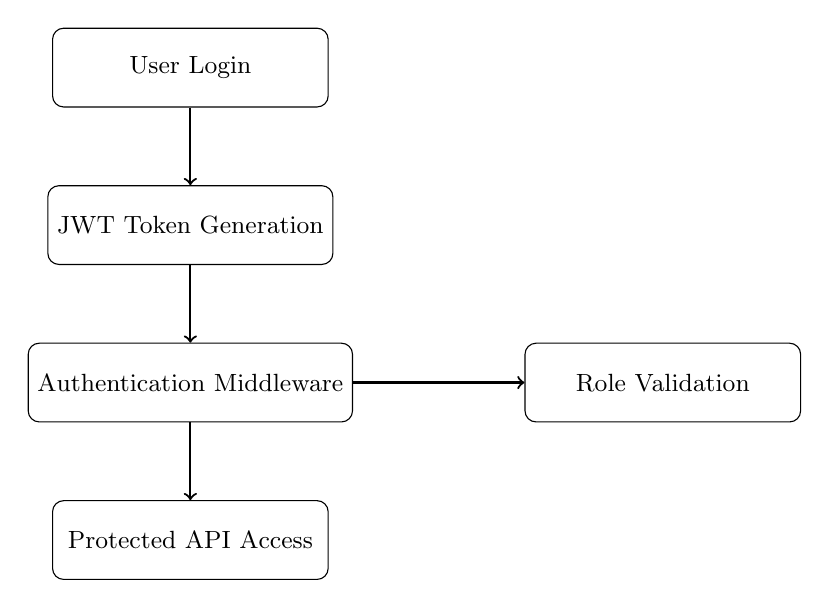
\begin{tikzpicture}[
node distance=2cm,
every node/.style={
draw,
rounded corners,
minimum width=3.5cm,
minimum height=1cm,
align=center,
font=\small
}
]
\node (login) {User Login};
\node (jwt) [below of=login] {JWT Token Generation};
\node (middleware) [below of=jwt] {Authentication Middleware};
\node (api) [below of=middleware] {Protected API Access};
\node (roles) [right of=middleware, xshift=4cm] {Role Validation};
\draw[->, thick] (login) -- (jwt);
\draw[->, thick] (jwt) -- (middleware);
\draw[->, thick] (middleware) -- (api);
\draw[->, thick] (middleware) -- (roles);
\end{tikzpicture}
\caption{JWT Authentication Flow}
\label{fig:jwt-backend-flow}
\end{figure}

Authentication relies on JSON Web Tokens (JWT) to support a stateless API architecture. During authentication, the backend hashes incoming passwords using BCrypt and compares them against the stored hash. If valid, the system generates an access token with a 15-minute lifespan and a cryptographically signed refresh token stored in an HttpOnly cookie to mitigate cross-site scripting (XSS) risks. When the short-lived access token expires, the client proxy automatically submits the refresh token to obtain a new access token, preventing session disruption while minimizing the impact of a compromised access token. Role validation is performed during this middleware pass, blocking farmers from accessing officer endpoints.

% ============================================================
\section{Verification Workflow}
\label{sec:verification-workflow}
% ============================================================

The seed verification workflow coordinates image validation, deep learning classification, text extraction, and database persistence, as shown in Figure~\ref{fig:verification-workflow}.

\begin{figure}[H]
\centering
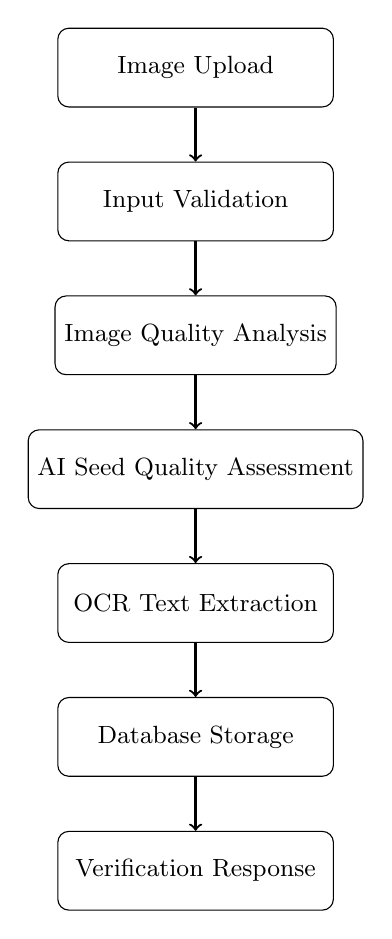
\begin{tikzpicture}[
node distance=1.7cm,
every node/.style={
draw,
rounded corners,
minimum width=3.5cm,
minimum height=1cm,
align=center,
font=\small
}
]
\node (upload) {Image Upload};
\node (validation) [below of=upload] {Input Validation};
\node (quality) [below of=validation] {Image Quality Analysis};
\node (ai) [below of=quality] {AI Seed Quality Assessment};
\node (ocr) [below of=ai] {OCR Text Extraction};
\node (database) [below of=ocr] {Database Storage};
\node (response) [below of=database] {Verification Response};
\draw[->, thick] (upload) -- (validation);
\draw[->, thick] (validation) -- (quality);
\draw[->, thick] (quality) -- (ai);
\draw[->, thick] (ai) -- (ocr);
\draw[->, thick] (ocr) -- (database);
\draw[->, thick] (database) -- (response);
\end{tikzpicture}
\caption{Seed Verification Workflow}
\label{fig:verification-workflow}
\end{figure}

The seed verification workflow handles image validation, AI inference, and database persistence. When a farmer submits an image, the API controller validates the upload headers and checks for basic image quality, such as assessing if the image is too blurry or dark, which would yield inaccurate model classifications. If the check passes, the image is written to Azure Blob Storage, and the system concurrently calls the ResNet50 FastAPI classification endpoint and the Azure OCR text extraction API. Once both responses return, the system saves the classification scores, morphological parameters, and label text to SQL Server. Finally, the backend feeds these inputs to Azure OpenAI to generate a clear advisory report, returnable as a unified JSON response.

% ============================================================
% ============================================================
\section{Configuration and Deployment}
\label{sec:configuration-deployment}
% ============================================================

We split application configurations into environment-specific files: \texttt{appsettings.json}, \texttt{appsettings.Development.json}, and \texttt{appsettings.Production.json}. During local development, the app connects to a local database instance and disables HTTPS enforcement. In production, we override these settings using environment variables injected by our container hosting platform, securing our database credentials, JWT security keys, and Azure service passwords.

During startup, the \texttt{Program.cs} entry point reads these parameters to register database context classes, configure our dependency injection containers, enable JWT validation rules, and build the HTTP request pipeline. This allows us to run the application with minimal dependencies during local development and easily switch to cloud databases and monitoring in our production environment.
